\documentclass{article}

\usepackage{listings}
\usepackage{amsmath}
\usepackage{hyperref}
\usepackage{graphicx}

\hypersetup{
    colorlinks=false, %set true if you want colored links
    linktoc=all,     %set to all if you want both sections and subsections linked
    linkcolor=blue,  %choose some color if you want links to stand out
}

\lstset{
 frame=bt,
 %frameround=tttt,
%mathescape=true,
  %language=Java,
  breaklines=true,
  showstringspaces=false,
  columns=flexible,
  numbers=none,
  %commentstyle=\color{MidnightBlue},
 %stringstyle=\color{gray},
  %stringstyle=\color{purple},
  basicstyle=\footnotesize\ttfamily,
  %literate=*{\$}{{\textcolor{arsenic}{\$}}}{1},
  tabsize=4
}

\title{\textbf{Progetto di Ricerca Operativa} \\
	\large \textbf{Map Coloring (con variante) in AMPL} \\
}

\author{Vetere Francesco\\ Matricola n. 313336 \\ \texttt{(francesco.vetere@studenti.unipr.it)}}
\date{}

\renewcommand*\contentsname{Indice}

\begin{document}
\maketitle
\tableofcontents

\pagebreak

\section{Descrizione del problema} 

Il problema affrontato in questo progetto consiste nell'implementazione in linguaggio \texttt{AMPL} del problema del \texttt{Map Coloring}, e di una sua interessante variante.\\
Risolvere il problema del \texttt{Map Coloring} significa assegnare ad ogni regione di una mappa geografica un colore, in modo tale che due regioni confinanti abbiano sempre colori diversi. Il numero di colori cercato \'e ovviamente quello minimo (utilizzando sempre un numero di colori pari al numero di regioni infatti, il problema diventerebbe banale).\\
La mappa geografica pu\'o essere rappresentata tramite un grafo $G = (V, E)$ in cui:
\begin{itemize}
\item $V=\{v_{1},...,v_{n}\}$ rappresenta l'insieme delle \emph{n} regioni della mappa geografica;
\item $E=\{(v_{i}, v_{j}) : v_{i}, v_{j} \in V, v_{i} \neq v_{j}\}$, dove $ (v_{i}, v_{j}) = 1 \iff \: v_{i}, v_{j} \; confinanti$ rappresenta l'insieme delle coppie di regioni \emph{i} e \emph{j} che sono confinanti sulla mappa geografica.
\end{itemize}

Una variante del problema appena descritto consiste nel cercare di eliminare un numero di regioni minimo in modo tale che la mappa risulti colorabile con un certo numero $k$ di colori. Anche in questa variante \'e subito evidente come prendendo $k = |V|$ il problema diventi banale.\\

Nel seguito di questo elaborato, si indicheranno con \texttt{map\_coloring} e \texttt{map\_coloring\_2} rispettivamente il primo problema ed il secondo.
\pagebreak

\section{Modelli matematici}
Come visto nella descrizione generale dei problemi, viene utilizzata una rappresentazione mediante grafo per la mappa geografica.\\
I modelli utilizzeranno dunque 3 insiemi:
\begin{itemize}
	\item[$\bullet$] $NODES$: L'insieme dei nodi (ogni nodo \'e una regione della mappa)\\
	\item[$\bullet$] $EDGES$: L'insieme degli archi (un arco (\emph{i}, \emph{j}) indica che le regioni \emph{i} e \emph{j} sono confinanti)\\
	\item[$\bullet$] $COLORS$: L'insieme dei colori (come si vedr\'a in seguito, di cardinalit\'a sufficientemente elevata)\\
	\end{itemize}
	
Vengono di seguito mostrati i modelli matematici per i due problemi.\\

\subsection{map\_coloring}
Per quanto riguarda \texttt{map\_coloring}, le componenti del modello sono:\\

\begin{itemize}
\item[] \textsc{variabili}
	\begin{itemize}
	\item[$\bullet$] $node\_color_{n,c}$: ad ogni coppia nodo $n$ e colore $c$ associamo una variabile binaria $node\_color_{n,c}$ che ha valore 1 se al nodo $n$ \'e assegnato il colore $c$, 0 altrimenti.\\
	\item[$\bullet$] $color\_used_{c}$: ad ogni colore $c$ associamo una variabile binaria $color\_used_{c}$ che ha valore 1 se il colore $c$ \'e stato utilizzato, 0 altrimenti.\\
	\end{itemize}
	
\item[] \textsc{vincoli}
	\begin{itemize}
	\item[$\bullet$] Un primo vincolo consiste nel richiedere che ad ogni nodo sia assegnato un solo colore:\\
	\begin{equation*}
	\begin{aligned}
	& & &  \sum\limits_{c \in COLORS} node\_color_{n,c} = 1 & \forall n \in NODES\\ 
	
	\end{aligned}
	\end{equation*}

	
	\item[$\bullet$] Il secondo vincolo impone che non vi siano due nodi adiacenti aventi lo stesso colore assegnato:\\
	\begin{equation*}
	\begin{aligned}
	& & &  node\_color_{i,c} + node\_color_{j,c} \le color\_used_{c} & \forall (i,j) \in EDGES, \forall c \in COLORS\\
		
	\end{aligned}
	\end{equation*}

	
	\item[$\bullet$] Gli ultimi due vincoli impongono le condizioni di interezza sulle variabili:\\
	\begin{equation*}
	\begin{aligned}
	& & &  node\_color_{i,c} \in \{0, 1\} & \forall i \in NODES, \forall c \in COLORS\\
	& & &  color\_used_{c} \in \{0, 1\} & \forall c \in COLORS\\
	
	\end{aligned}
	\end{equation*}

	
	\end{itemize}


\item[] \textsc{obiettivo} 
	\begin{itemize}
	\item[$\bullet$] L'obiettivo consiste nel minimizzare il numero di colori utilizzati:\\
	\begin{equation*}
	\begin{aligned}
	& {\text{min}} & & \sum\limits_{c \in COLORS} color\_used_{c}\\
	
	\end{aligned}
	\end{equation*}

	
	\end{itemize}
\end{itemize}

Il modello matematico completo risulta essere quindi il seguente:\\

\begin{equation*}
\begin{aligned}
& {\text{min}} & & \sum\limits_{c \in COLORS} color\_used_{c} \\
& & &  \sum\limits_{c \in COLORS} node\_color_{n,c} = 1 & \forall n \in NODES\\ 
& & &  node\_color_{i,c} + node\_color_{j,c} \le color\_used_{c} & \forall (i,j) \in EDGES, \forall c \in COLORS\\
& & &  node\_color_{i,c} \in \{0, 1\} & \forall i \in NODES, \forall c \in COLORS\\
& & &  color\_used_{c} \in \{0, 1\} & \forall c \in COLORS\\

\end{aligned}
\end{equation*}

Notiamo che il problema di Programmazione Matematica appena descritto contiene solamente variabili binarie, ricadendo dunque nella classe dei problemi di Programmazione Binaria Intera (PBI). Ci aspettiamo dunque che, nel caso generale, il problema sia NP-completo.\\

\pagebreak

\subsection{map\_coloring\_2}
Per quanto riguarda \texttt{map\_coloring\_2}, le componenti del modello sono quasi identiche a quelle viste per \texttt{map\_coloring}, con pochi accorgimenti in pi\'u:\\

\begin{itemize}
\item[] \textsc{variabili}
	\begin{itemize}
	\item[$\bullet$] $node\_color_{n,c}$: ad ogni coppia nodo $n$ e colore $c$ associamo una variabile binaria $node\_color_{n,c}$ che ha valore 1 se al nodo $n$ \'e assegnato il colore $c$, 0 altrimenti.\\
	\item[$\bullet$] $color\_used_{c}$: ad ogni colore $c$ associamo una variabile binaria $color\_used_{c}$ che ha valore 1 se il colore $c$ \'e stato utilizzato, 0 altrimenti.\\
	\item[$\bullet$] $node\_deleted_{n}$: ad ogni nodo $n$ associamo una variabile binaria $node\_deleted_{n}$ che ha valore 1 se il nodo $n$ \'e stato eliminato (non colorato), 0 altrimenti.\\
	\end{itemize}
	
\item[] \textsc{vincoli}
	\begin{itemize}
	\item[$\bullet$] Un primo vincolo consiste nel richiedere che ad ogni nodo sia assegnato un solo colore, tenendo per\'o in considerazione anche il fatto che alcuni nodi potrebbero essere stati eliminati e dunque non avere alcun colore assegnato:\\
	\begin{equation*}
	\begin{aligned}
	& & &  \sum\limits_{c \in COLORS} node\_color_{n,c} = 1 - node\_deleted_{n} & \forall n \in NODES\\ 
	\end{aligned}
	\end{equation*}
	
	Notiamo infatti che nel caso in cui il nodo non sia stato eliminato, il vincolo coincide esattamente con l'analogo vincolo considerato in \texttt{map\_coloring}. In caso contrario, il vincolo impone che per tale nodo non vi sia alcun colore assegnato.\\
	
	\item[$\bullet$] Il secondo vincolo impone che non vi siano due nodi adiacenti aventi lo stesso colore assegnato:\\
	\begin{equation*}
	\begin{aligned}
	& & &  node\_color_{i,c} + node\_color_{j,c} \le color\_used_{c} & \forall (i,j) \in EDGES, \forall c \in COLORS\\
	
	\end{aligned}
	\end{equation*}
	
	\item[$\bullet$] Gli ultimi tre vincoli impongono le condizioni di interezza sulle variabili:\\
	\begin{equation*}
	\begin{aligned}
	& & &  node\_color_{i,c} \in \{0, 1\} & \forall i \in NODES, \forall c \in COLORS\\
	& & &  color\_used_{c} \in \{0, 1\} & \forall c \in COLORS\\
	& & &  node\_deleted_{n} \in \{0, 1\} & \forall n \in NODES\\
	
	\end{aligned}
	\end{equation*}
	
	\end{itemize}

\item[] \textsc{obiettivo} 
	\begin{itemize}
	\item[$\bullet$] L'obiettivo consiste nel minimizzare il numero di nodi eliminati:\\
	\begin{equation*}
	\begin{aligned}
	& {\text{min}} & & \sum\limits_{n \in NODES} node\_deleted_{n} \\
	\end{aligned}
	
	\end{equation*}
	
	\end{itemize}

\end{itemize}

Il modello matematico completo risulta essere quindi il seguente:\\

\begin{equation*}
\begin{aligned}
& {\text{min}} & & \sum\limits_{n \in NODES} node\_deleted_{n} \\
& & &  \sum\limits_{c \in COLORS} node\_color_{n,c} = 1 - node\_deleted_{n} & \forall n \in NODES\\ 
& & &  node\_color_{i,c} + node\_color_{j,c} \le color\_used_{c} & \forall (i,j) \in EDGES, \forall c \in COLORS\\
& & &  node\_color_{i,c} \in \{0, 1\} & \forall i \in NODES, \forall c \in COLORS\\
& & &  color\_used_{c} \in \{0, 1\} & \forall c \in COLORS\\
& & &  node\_deleted_{n} \in \{0, 1\} & \forall n \in NODES\\

\end{aligned}
\end{equation*}

Anche in questo caso notiamo ovviamente che il problema \'e ancora un problema di Programmazione Binaria Intera (PBI).\\

\pagebreak

\section{Modelli AMPL}
Vengono di seguito mostrati i file \texttt{.mod} per il linguaggio \texttt{AMPL}.\\

\subsection{map\_coloring.mod}
\texttt{map\_coloring.mod}
\lstinputlisting{map_coloring.mod}

\vspace{5mm}

Il file modella in linguaggio \texttt{AMPL} quanto visto nell'analogo modello matematico.\\
Per prima cosa vengono dichiarati gli insiemi che caratterizzano il problema: \texttt{NODES} e \texttt{EDGES} descrivono il grafo (\texttt{EDGES} \'e contenuto nel prodotto cartesiano \texttt{NODES} $\times$ \texttt{NODES}), mentre \texttt{COLORS} \'e l'insieme contenente i colori assegnabili.\\

Seguono poi le dichiarazioni delle variabili \texttt{node\_color} e \texttt{color\_used}.\\
La prima modella un array bidimensionale avente indici sull'insieme dei nodi e dei colori, in cui ogni valore, vincolato ad essere di tipo binario, indica se un particolare nodo \'e assegnato ad un particolare colore o meno.\\

La seconda modella un array monodimensionale avente indici sull'insieme dei colori, con valori ancora binari che indicano se un particolare colore \'e stato scelto per l'assegnamento o meno.\\ 

Vengono dichiarati poi i due vincoli che caratterizzano il problema: \texttt{one\_color\_per\_node} e \texttt{different\_color\_adjacent}.\\
La prima dichiarazione genera tanti vincoli quanti sono gli elementi dell'insieme \texttt{NODES}. Ogni vincolo generato impone che, per quel particolare nodo, la somma dei colori assegnati sia esattamente pari a 1 (questo per evitare assegnamenti di 0 oppure 2 colori per un singolo nodo).\\
La seconda dichiarazione genera un vincolo per ogni elemento dell'insieme formato dal prodotto cartesiano di \texttt{EDGES} e \texttt{COLORS}. Ogni vincolo generato impone che due nodi adiacenti non possano essere assegnati allo stesso colore (altrimenti si avrebbe una colorazione non valida).\\

Viene infine esplicitato l'obiettivo \texttt{num\_colors}, che semplicemente minimizza la somma di tutti i colori utilizzati.\\
\pagebreak

\subsection{map\_coloring\_2.mod}
\texttt{map\_coloring\_2.mod}
\lstinputlisting{map_coloring_2.mod}

\vspace{5mm}

Questa variante \'e molto simile al problema originale.\\
Viene introdotta una nuova variabile, \texttt{node\_deleted}, che modella un array monodimensionale avente indici sull'insieme dei nodi, con valori binari che indicano se un nodo sia stato eliminato o meno.\\

Cambia anche il vincolo \texttt{one\_color\_per\_node}: per ogni nodo, \'e richiesto che la somma dei colori assegnati sia ora pari a \texttt{1 - node\_deleted[n]}, per tenere conto del fatto che ora il solver ha la facolt\'a di scegliere che un nodo venga escluso dalla colorazione.\\

Anche l'obiettivo \'e differente: \texttt{min\_deleted} richiede infatti che sia minimizzata la somma dei nodi eliminati.\\
\pagebreak

\section{Esempi di esecuzione}
Vengono ora analizzati alcuni esempi di file \texttt{.dat} per entrambi i problemi.\\
Per testare l'esecuzione dei modelli corredati dai loro dati, si utilizza un file \texttt{.run} di questo tipo:\\

\texttt{map\_coloring.run}
\lstinputlisting{map_coloring.run}

\vspace{5mm}

\texttt{map\_coloring\_2.run}
\lstinputlisting{map_coloring_2.run}

\vspace{5mm}

Come si pu\'o notare, \'e stato scelto di mostrare in output il contenuto delle variabili al termine della risoluzione da parte del solver, in modo da poter trarre alcune conclusioni sui risultati ottenuti.\\

\subsection{map\_coloring}
\subsubsection{map\_coloring\_es1.dat}

Per quanto riguarda \texttt{map\_coloring}, analizziamo intanto il caso di un grafo completo con $|V| = 5$, ossia un grafo in cui ogni vertice \'e collegato tramite un arco agli altri 4 vertici restanti. \\
Sebbene questa situazione non rappresenti una mappa, in quanto vale un teorema per cui non \'e possibile dividere un piano in 5 regioni in modo che ciascuna tocchi le altre 4 (il confine tra le regioni \'e da intendersi come un tratto di territorio, e non semplicemente come uno o pi\'u punti separati: in tal caso infatti, sarebbe sufficiente considerare una circonferenza e dividerla in spicchi, ed allora tutti gli spicchi sarebbero confinanti tra di loro), \'e comunque un caso interessante da analizzare.\\

Sia dato quindi il seguente grafo:\\

\begin{center}
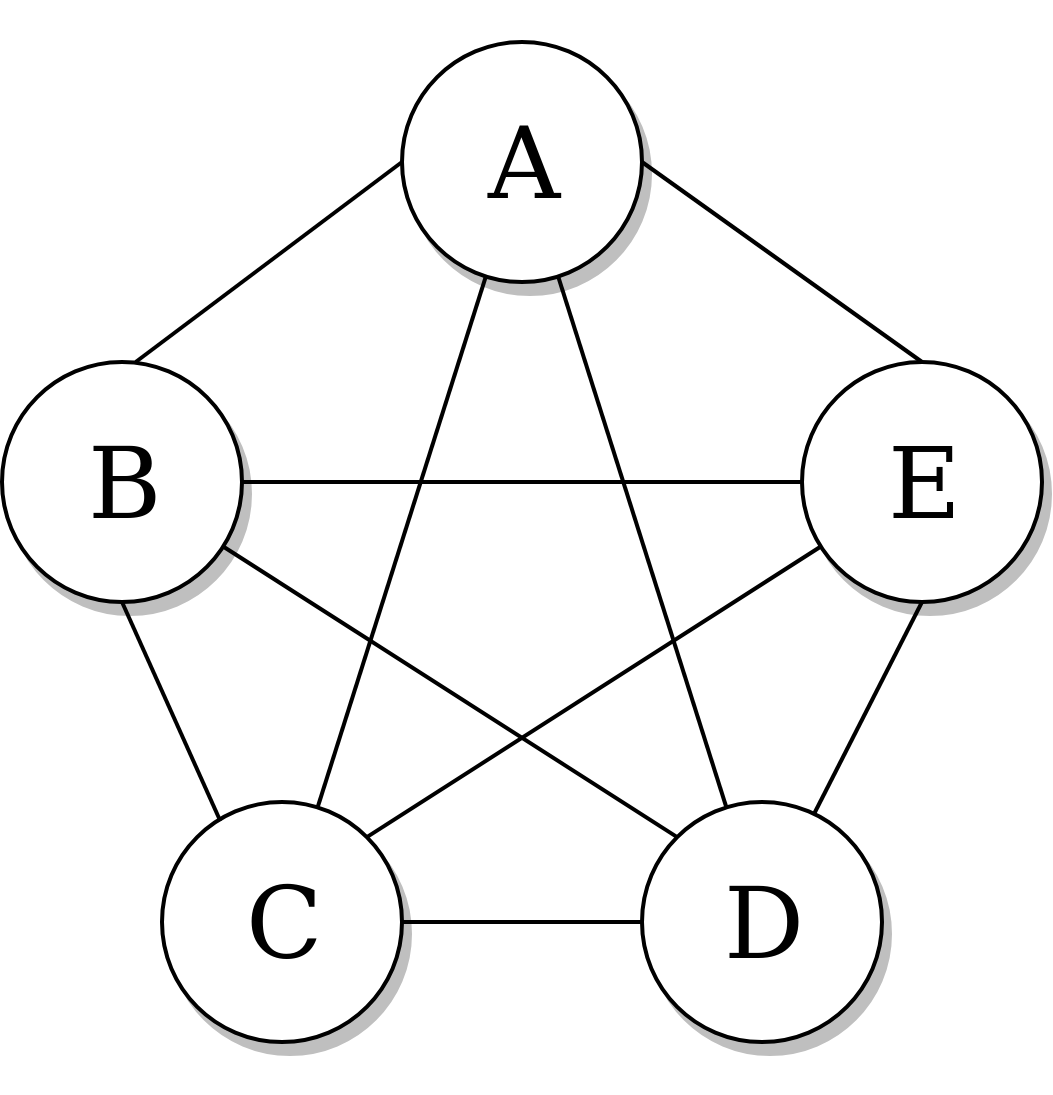
\includegraphics[scale=0.15]{complete_graph.png}
\end{center}

Il file \texttt{.dat} che implementa questa situazione \'e il seguente:

\vspace{5mm}
\texttt{map\_coloring\_es1.dat}
\lstinputlisting{map_coloring_dat/map_coloring_es1.dat}
\vspace{5mm}

Si noti che \'e fondamentale definire un numero di colori sufficientemente elevato per poter ottenere una soluzione ammissibile del problema: un upper bound sicuramente valido \'e dato dal numero di nodi presenti nel grafo. La teoria ci dice in realt\'a che ogni mappa ammette una colorazione valida formata da 4 soli colori, ma non essendo questa una mappa tale risultato non vale.\\
Ad ogni modo anche nei successivi esempi ignoreremo questo teorema, dando al solver pi\'u colori disponibili di quelli effettivamente necessari, al fine di poter osservare come certi colori vengano esclusi.\\

\pagebreak

Dopo aver lanciato \texttt{map\_coloring.run} si ottiene il seguente risultato:\\

\begin{verbatim}
Gurobi 8.1.0: optimal solution; objective 5
6 simplex iterations
node_color [*,*]
: blue green orange red yellow    :=
A   0     0     0     1    0
B   0     0     0     0    1
C   0     0     1     0    0
D   0     1     0     0    0
E   1     0     0     0    0
;

color_used [*] :=
  blue  1
 green  1
orange  1
   red  1
yellow  1
;
\end{verbatim}

Notiamo che il solver trova una soluzione ottima eseguendo 6 iterazioni dell'algoritmo del simplesso.\\
Il valore ottimo, ossia 5, era in questo caso facilmente prevedibile: trattandosi di un grafo completo, ogni nodo \'e adiacente ai restanti $|V| - 1$ nodi: questo implica il fatto che ad ogni nodo dovr\'a necessariamente essere assegnato un colore differente.\\
Il contenuto delle variabili ci conferma quanto ipotizzato: la variabile \texttt{node\_color} mostra che ad ogni nodo \'e assegnato esattamente un colore (questo deve essere vero per qualsiasi tipo di grafo, a causa del vincolo \texttt{one\_color\_per\_node}) mentre la variabile \texttt{color\_used} mostra che effettivamente tutti i colori sono stati utilizzati.\\

\pagebreak

La soluzione ottima trovata dal solver \'e la seguente:\\

\begin{center}
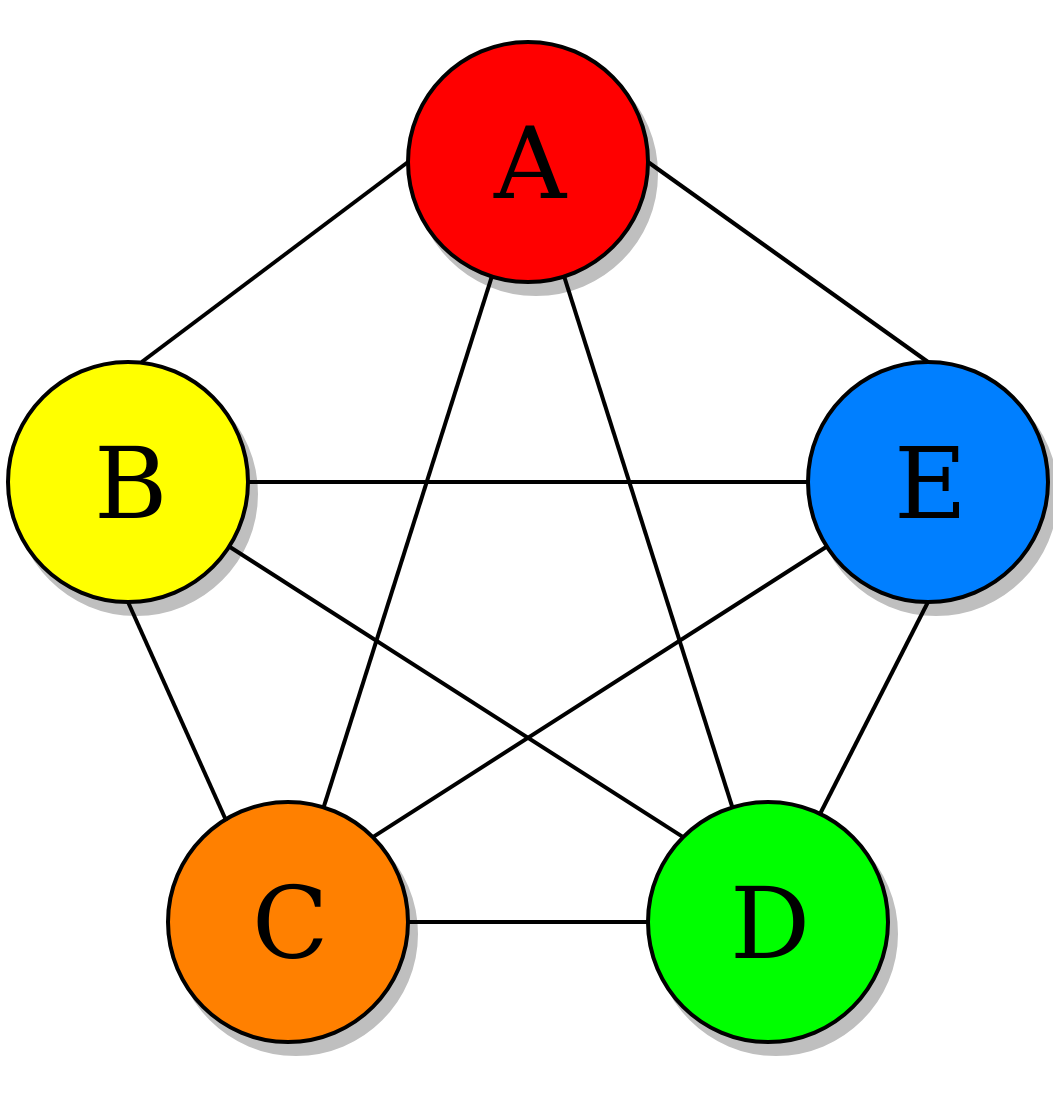
\includegraphics[scale=0.15]{complete_graph_coloured1.png}
\end{center}

\vspace{10mm}

\subsubsection{map\_coloring\_es2.dat}
Analizziamo ora il caso di un grafo non completo, come illustrato dalla seguente immagine:\\

\begin{center}
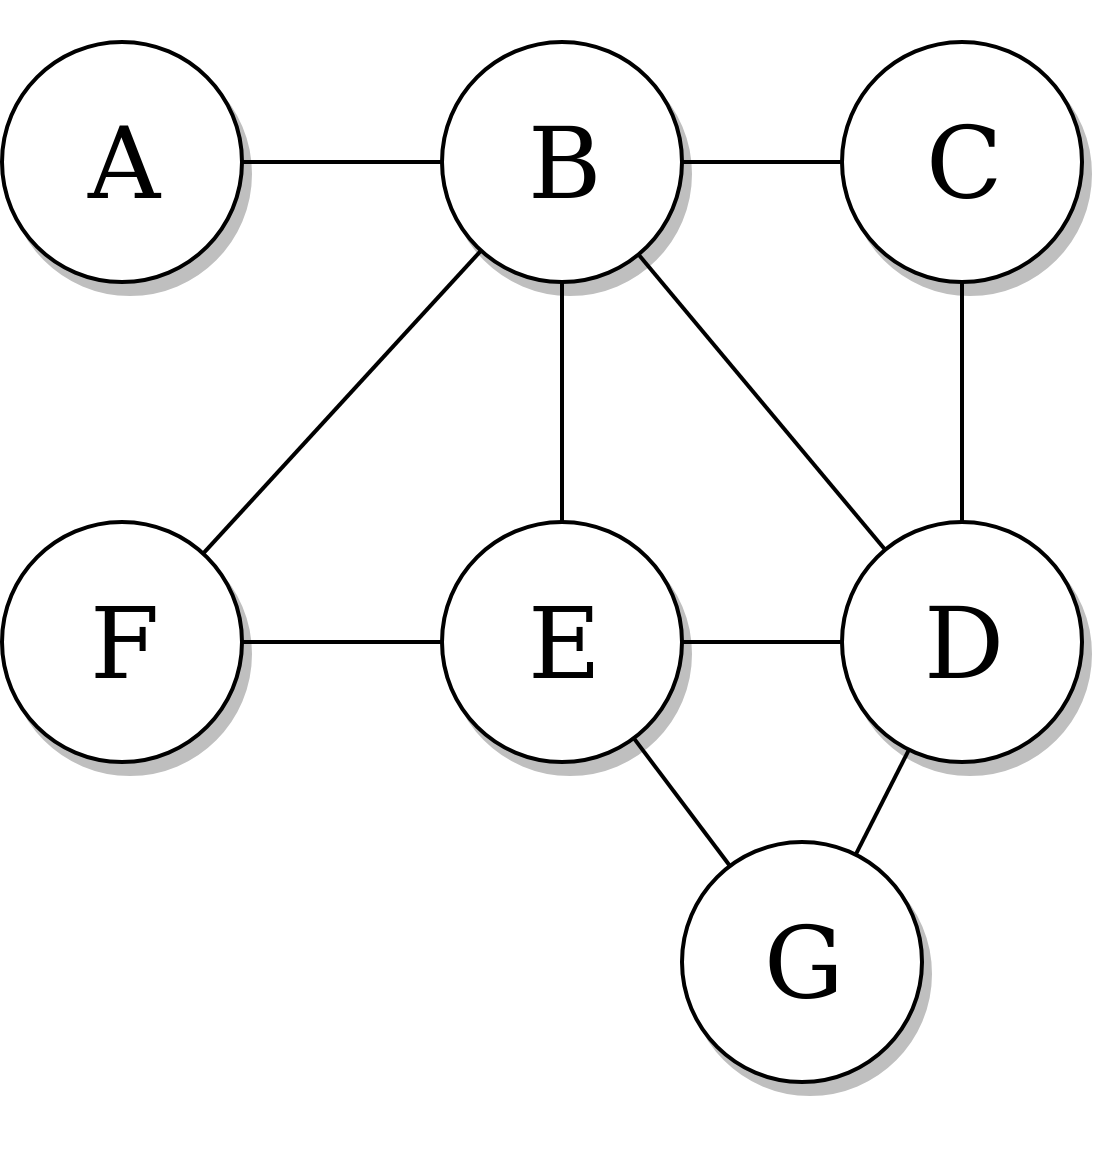
\includegraphics[scale=0.15]{non_complete_graph.png}
\end{center}

\pagebreak

Il file \texttt{.dat} che implementa questa situazione \'e il seguente:\\

\vspace{5mm}
\texttt{map\_coloring\_es2.dat}
\lstinputlisting{map_coloring_dat/map_coloring_es2.dat}
\vspace{5mm}

Dopo aver lanciato \texttt{map\_coloring.run} si ottiene il seguente risultato:\\
\begin{verbatim}
Gurobi 8.1.0: optimal solution; objective 3
30 simplex iterations
node_color [*,*]
: blue green orange red yellow    :=
A   0     0     0     0    1
B   0     1     0     0    0
C   1     0     0     0    0
D   0     0     0     0    1
E   1     0     0     0    0
F   0     0     0     0    1
G   0     1     0     0    0
;

color_used [*] :=
  blue  1
 green  1
orange  0
   red  0
yellow  1
;
\end{verbatim}

Notiamo che il solver trova una soluzione ottima eseguendo 30 iterazioni dell'algoritmo del simplesso.\\
Come evidente dal valore ottimo, il numero minimo di colori per ottenere una colorazione valida per il grafo \'e 3.\\
Utilizzando infatti i colori \texttt{blue}, \texttt{green} e \texttt{yellow}, notiamo che il solver riesce correttamente ad assegnare ad ogni nodo uno ed un solo colore, come richiesto dal problema.\\
La soluzione ottima trovata dal solver \'e rappresentata dalla seguente immagine:\\

\begin{center}
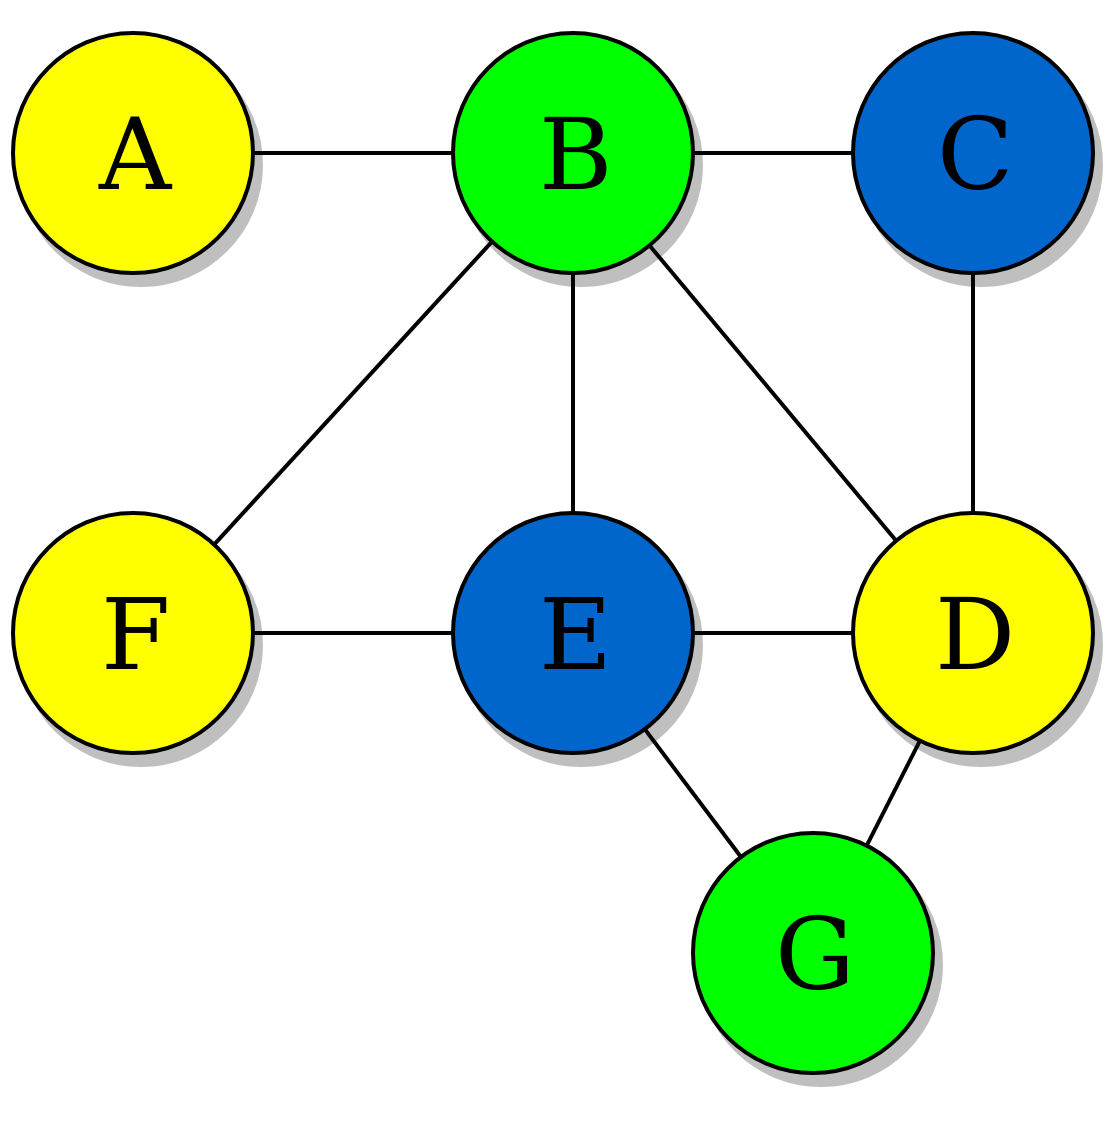
\includegraphics[scale=0.15]{non_complete_graph_coloured1.png}
\end{center}

\vspace{10mm}

\subsection{map\_coloring\_2}
\subsubsection{map\_coloring\_2\_es1.dat}
Per quanto riguarda \texttt{map\_coloring\_2}, analizziamo intanto il caso del grafo completo considerato in \texttt{map\_coloring}:\\

\begin{center}
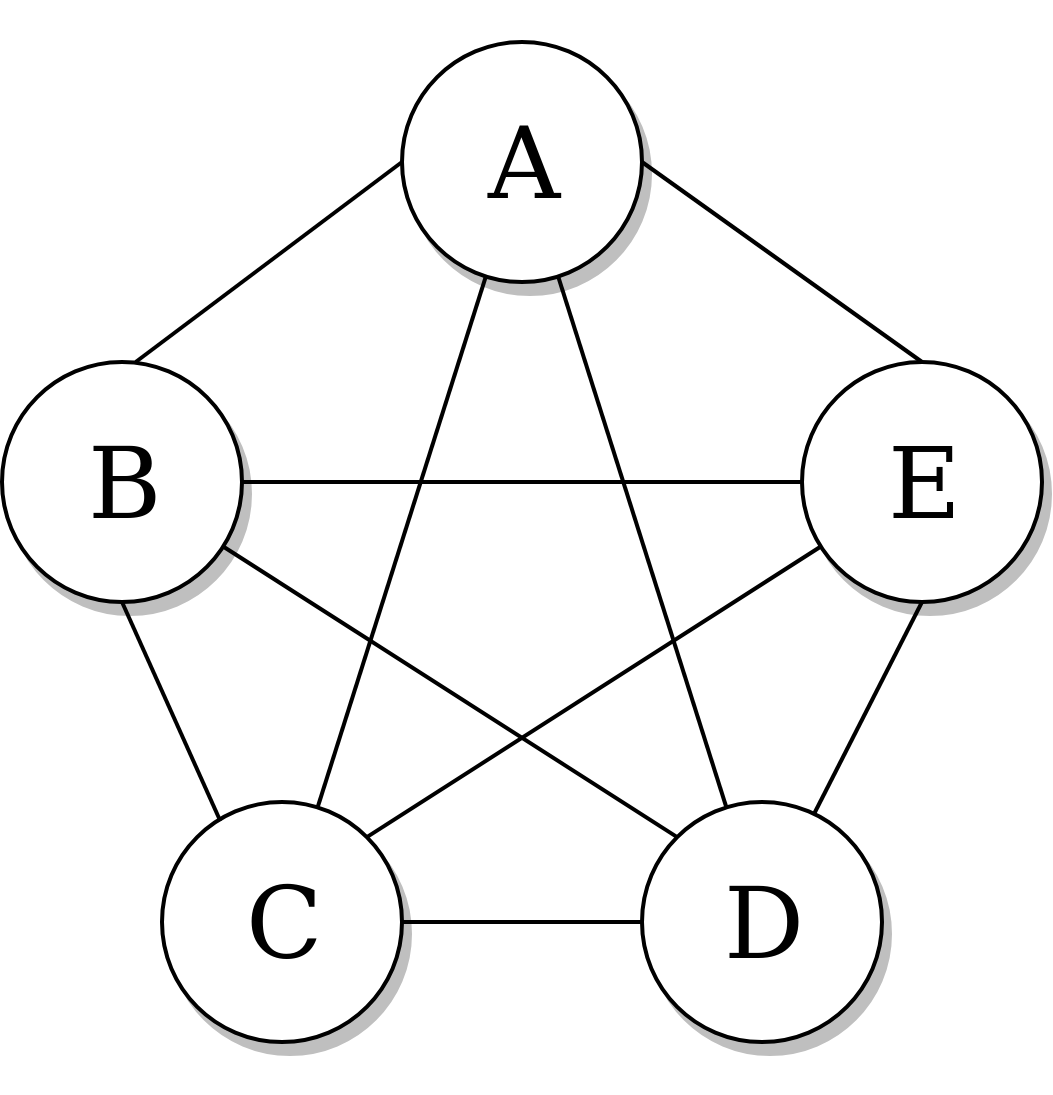
\includegraphics[scale=0.15]{complete_graph.png}
\end{center}

Lasciando invariato il numero di colori (ossia 5), si ha che banalmente il solver non elimina alcun nodo, poich\'e 5 \'e gi\'a il numero  minimo di colori per cui il grafo \'e colorabile.\\

\pagebreak

Il file \texttt{.dat} associato a questa situazione \'e lo stesso visto per \texttt{map\_coloring}:\\

\vspace{5mm}
\texttt{map\_coloring\_2\_es1.dat}
\lstinputlisting{map_coloring_2_dat/map_coloring_2_es1.dat}
\vspace{5mm}

Come previsto, il solver restituisce un output di questo tipo:\\

\begin{verbatim}
Gurobi 8.1.0: optimal solution; objective 0
9 simplex iterations
node_color [*,*]
: blue green orange red yellow    :=
A   0     0     0     0    1
B   0     1     0     0    0
C   0     0     1     0    0
D   1     0     0     0    0
E   0     0     0     1    0
;

color_used [*] :=
  blue  1
 green  1
orange  1
   red  1
yellow  1
;

node_deleted [*] :=
A  0
B  0
C  0
D  0
E  0
F  0
;

\end{verbatim}

\pagebreak 

Notiamo che la soluzione ottima \'e tuttavia diversa da quella precedente: questo \'e dovuto al fatto che ovviamente ci sono pi\'u combinazioni di assegnamenti nodo-colore che permettono di ottenere lo stesso valore obiettivo. La combinazione trovata dal solver \'e in questo caso infatti la seguente:\\

\begin{center}
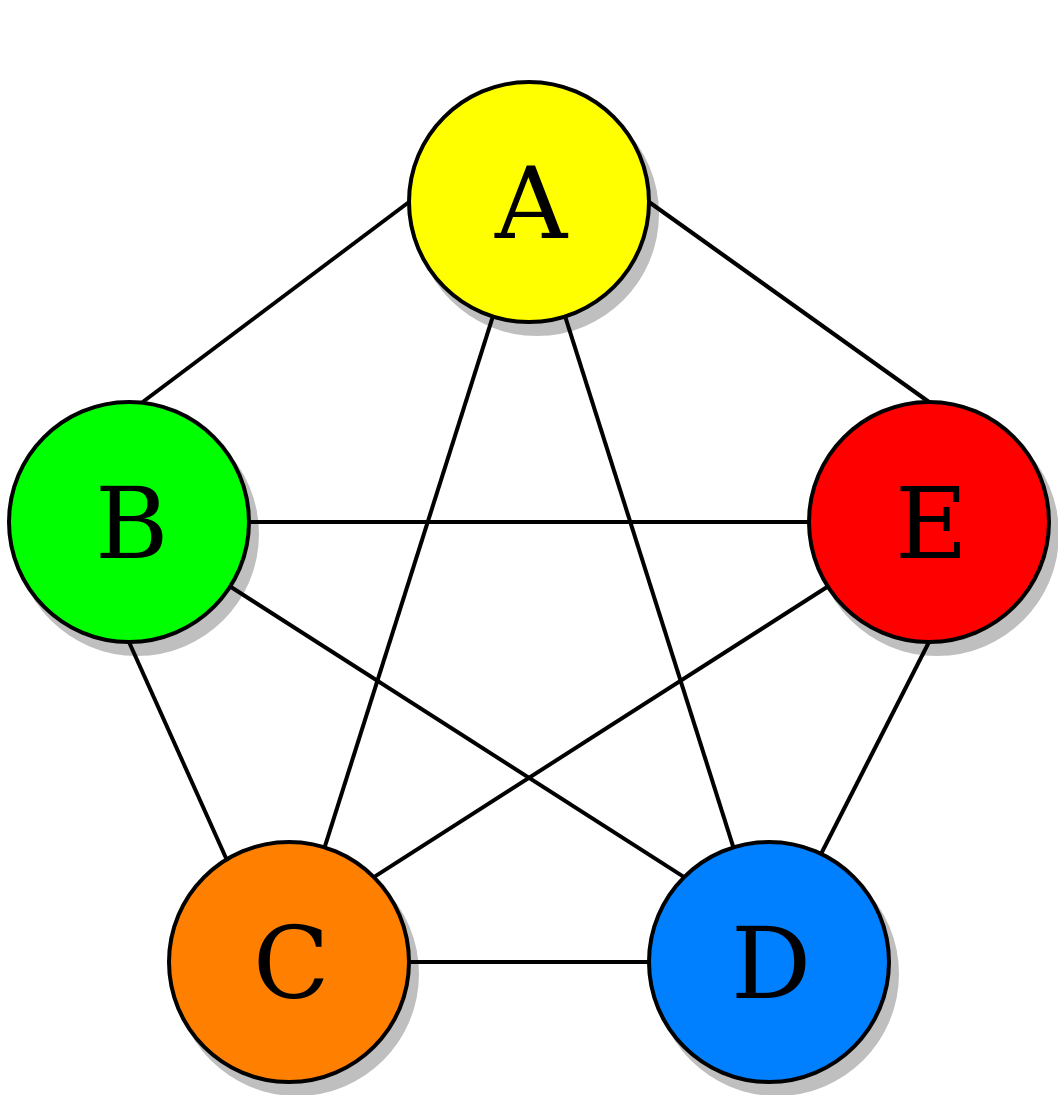
\includegraphics[scale=0.15]{complete_graph_coloured2.png}
\end{center}

\pagebreak

\subsubsection{map\_coloring\_2\_es2.dat}
Analizziamo ora il caso dello stesso grafo non completo considerato in \texttt{map\_coloring}:\\

\begin{center}
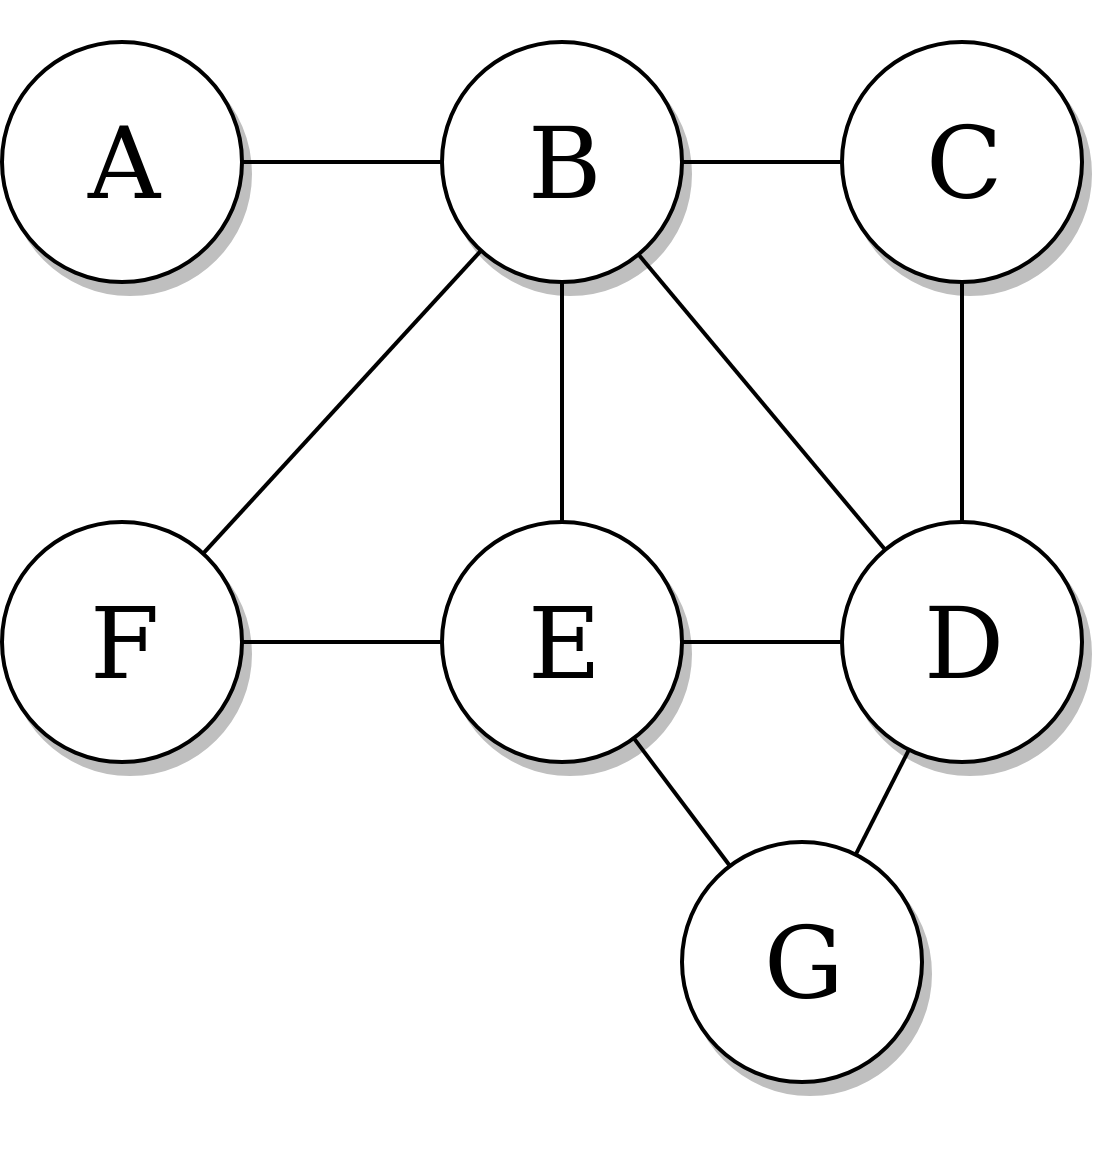
\includegraphics[scale=0.15]{non_complete_graph.png}
\end{center}

Dalla soluzione ottima ottenuta precedentemente, sappiamo che il grafo richiede un minimo di 3 colori per poter essere colorato in maniera ammissibile. Proviamo dunque a fissare un numero di colori $k = 2$: il solver, se possibile, dovr\'a scegliere di eliminare alcuni nodi al fine ottenere una colorazione valida.\\

Il file \texttt{.dat} che implementa questa situazione \'e il seguente:

\vspace{5mm}
\texttt{map\_coloring\_2\_es2.dat}
\lstinputlisting{map_coloring_2_dat/map_coloring_2_es2.dat}
\vspace{5mm}

\pagebreak

Dopo aver lanciato \texttt{map\_coloring\_2.run} si ottiene il seguente risultato:\\

\begin{verbatim}
Gurobi 8.1.0: optimal solution; objective 2
13 simplex iterations
1 branch-and-cut nodes
node_color :=
A blue   1
A red    0
B blue   0
B red    0
C blue   1
C red    0
D blue   0
D red    0
E blue   0
E red    1
F blue   1
F red    0
G blue   1
G red    0
;

color_used [*] :=
blue  1
 red  1
;

node_deleted [*] :=
A  0
B  1
C  0
D  1
E  0
F  0
G  0
;

\end{verbatim}

Notiamo che il solver riesce ad eliminare un certo numero di nodi al fine di ottenere una colorazione valida con soli 2 colori: una soluzione ottima \'e infatti trovata eseguendo 13 iterazioni dell'algoritmo del simplesso, utilizzato questa volta in combinazione con l'algoritmo branch and cut.\\

\pagebreak

Il valore ottimo \'e in questo caso 2: affinch\'e il grafo sia 2-colorabile, \'e necessario eliminare 2 nodi. Come evidenziato dal valore delle variabili, una possibile soluzione ottima consiste nell'eliminare i nodi \texttt{B} e \texttt{D}: cos\'i facendo, il grafo risultante \'e effettivamente 2-colorabile, e la soluzione ottima trovata dal solver \'e la seguente:\\

\begin{center}
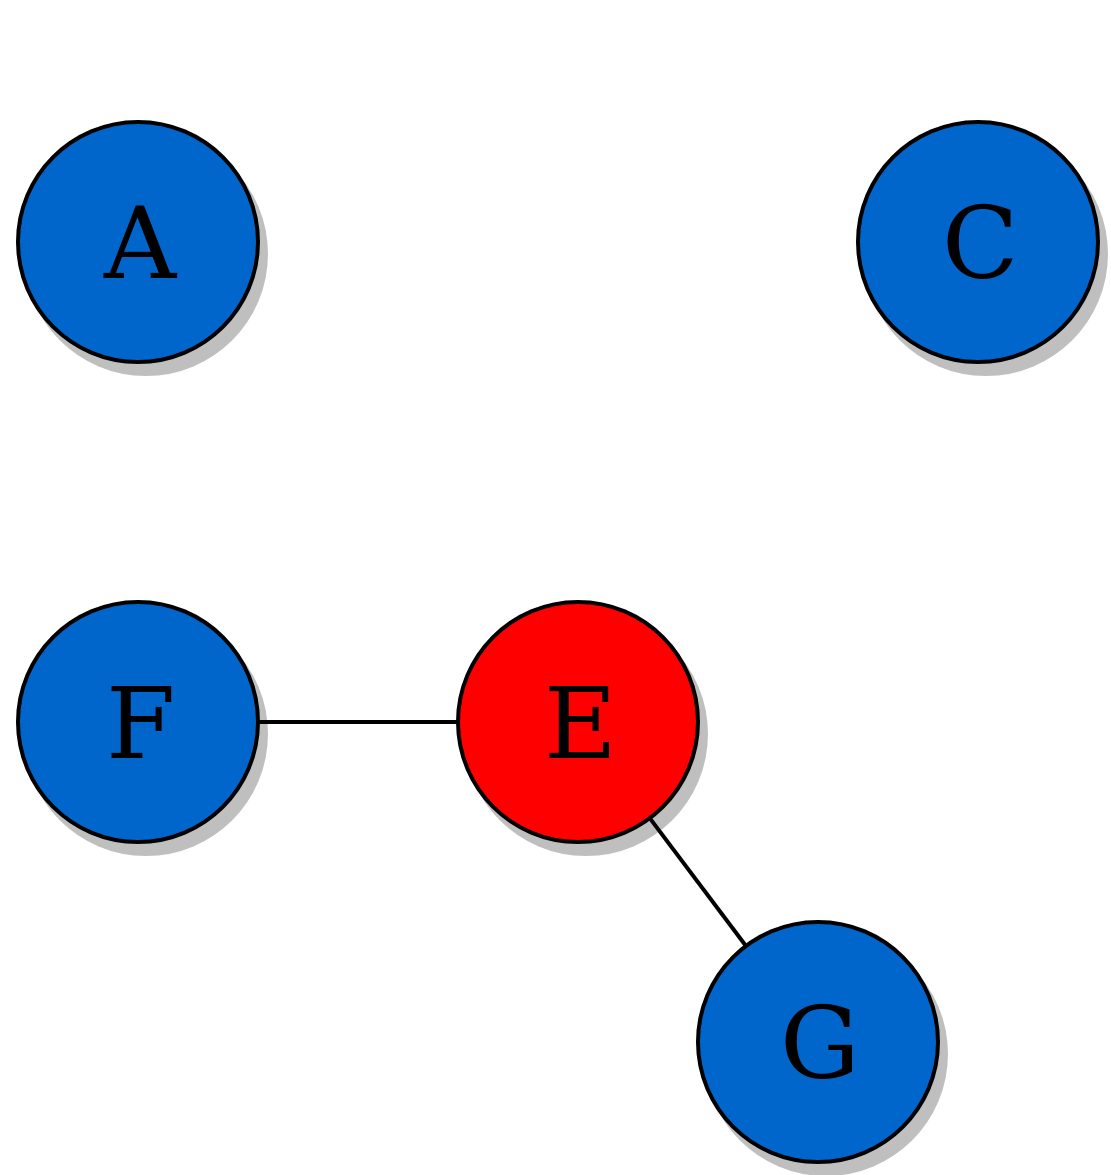
\includegraphics[scale=0.15]{non_complete_graph_coloured2.png}
\end{center}

\pagebreak

\subsubsection{map\_coloring\_2\_es3.dat}
Analizziamo ora il caso di un albero binario:\\

\begin{center}
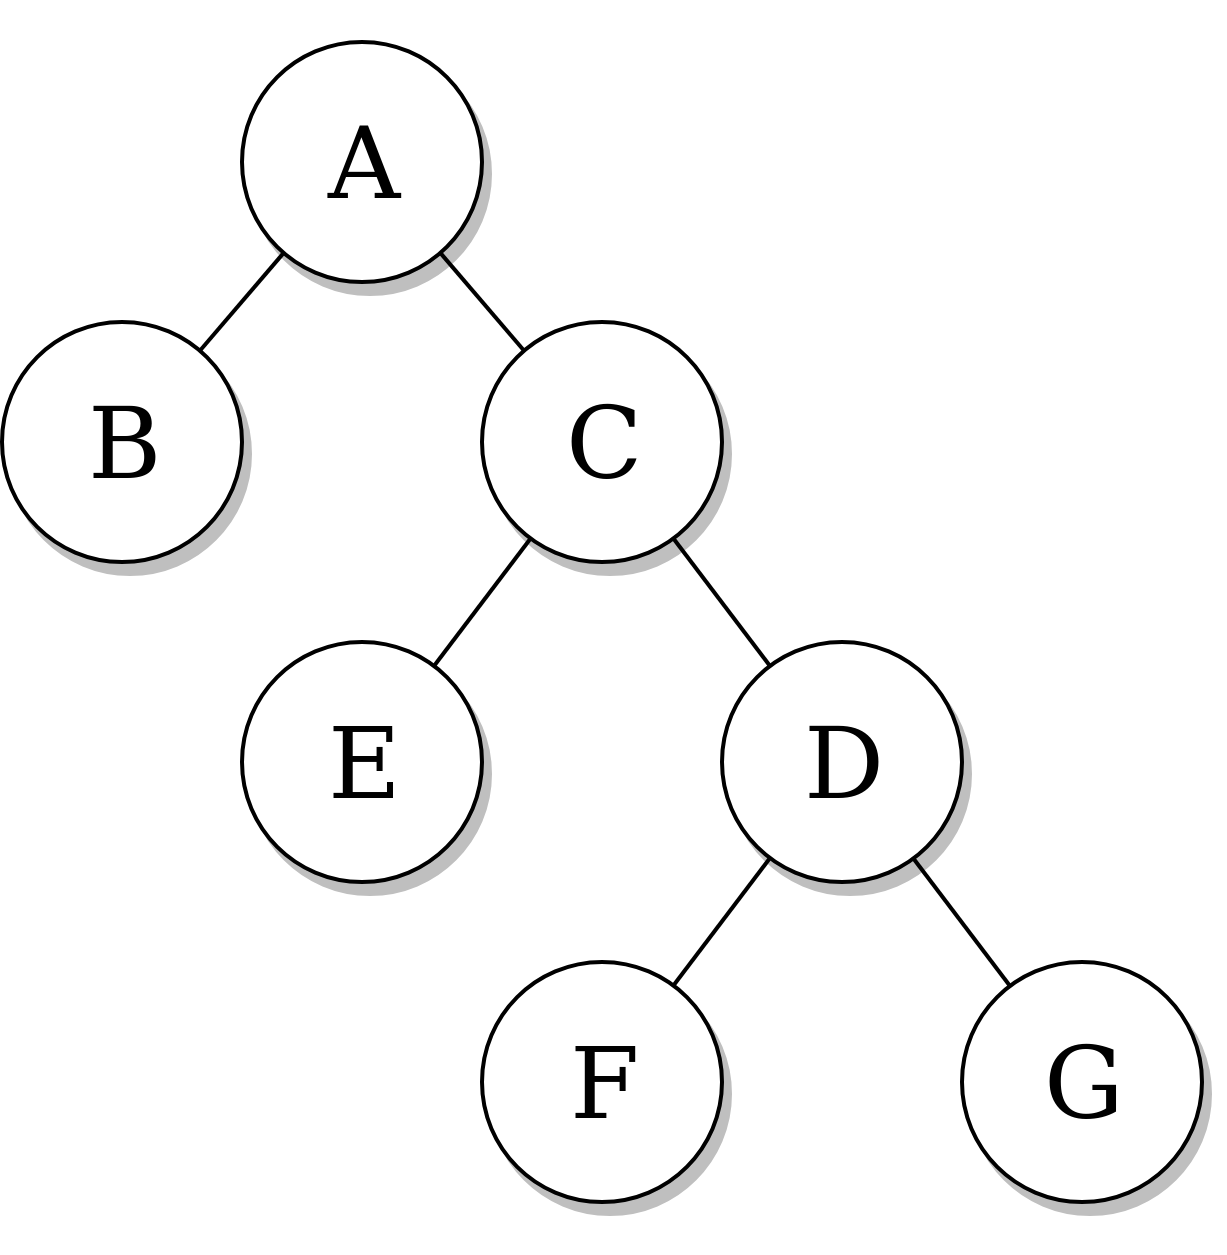
\includegraphics[scale=0.15]{tree.png}
\end{center}

\vspace{10mm}

In generale, un albero binario necessita di almeno 2 colori per poter essere colorabile. Analizziamo allora il comportamento del solver nel caso venga reso disponibile 1 solo colore, implementando il seguente file \texttt{.dat}:\\

\vspace{5mm}
\texttt{map\_coloring\_2\_es3.dat}
\lstinputlisting{map_coloring_2_dat/map_coloring_2_es3.dat}
\vspace{5mm}

\pagebreak

Dopo aver lanciato \texttt{map\_coloring\_2.run} si ottiene il seguente risultato:\\

\begin{verbatim}
Gurobi 8.1.0: optimal solution; objective 3
node_color :=
A red   0
B red   1
C red   0
D red   0
E red   1
F red   1
G red   1
;

color_used [*] :=
red  1
;

node_deleted [*] :=
A  1
B  0
C  1
D  1
E  0
F  0
G  0
;
\end{verbatim}

\pagebreak

Notiamo che il solver \'e costretto ad eliminare qualsiasi collegamento esistente tra i nodi: una soluzione ottima \'e quella di eliminare i nodi \texttt{A}, \texttt{C} e \texttt{D}.\\
Cos\'i facendo, il grafo risultante essere 1-colorabile (il solver sceglie l'unico colore disponibile, \texttt{red}):

\begin{center}
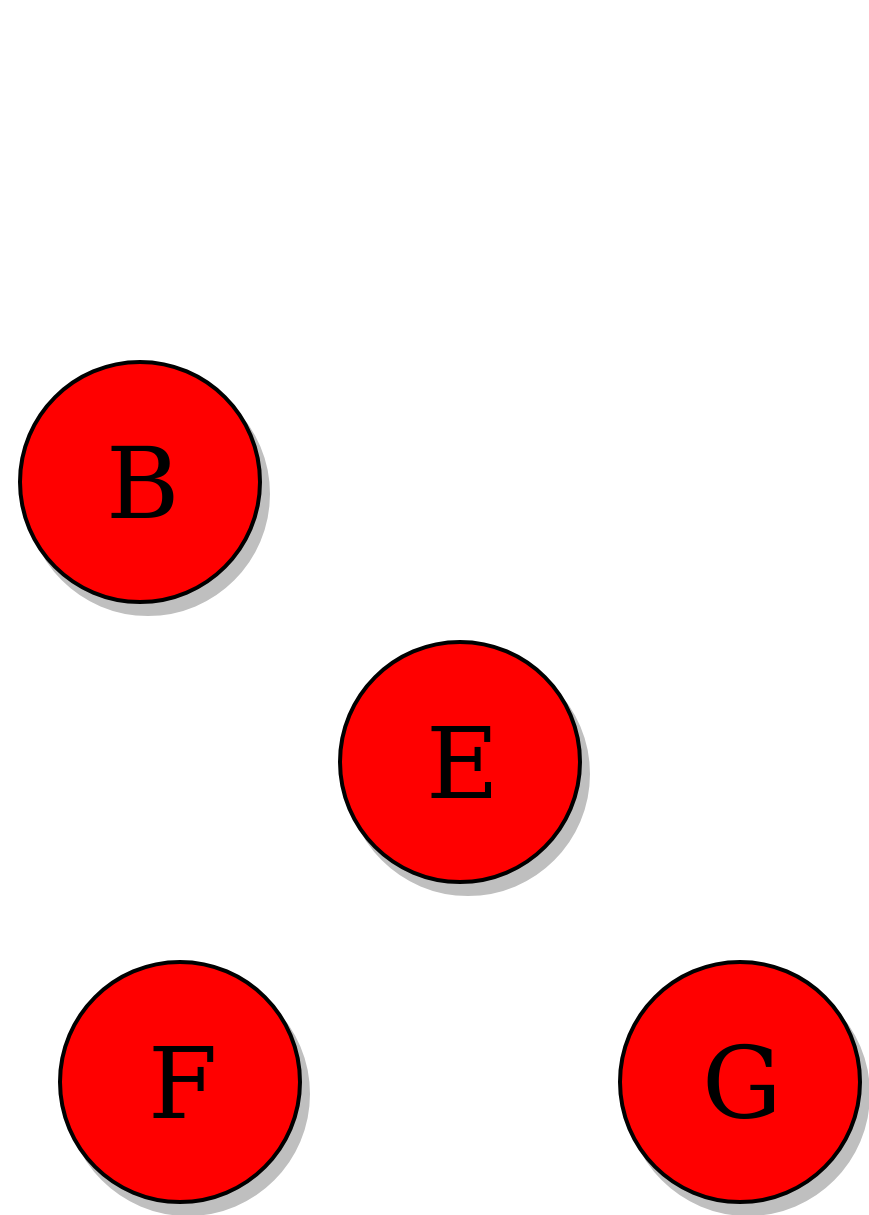
\includegraphics[scale=0.15]{tree_coloured.png}
\end{center}

\end{document}
